\chapter{Sizing}\label{cp:sizing}

\section{Wing and Tail}

The flight performance and structural worked together to generate the table of initial wing sizes shown in \autoref{tbl:initial_wing_sizing}.

\begin{table}[htpb]
    \centering
    \caption[Initial wing sizing]{Initial wing sizing parameters.}
    \begin{tabular}{ccc}
        \toprule
        \textbf{Name} & \textbf{Variable} & \textbf{Dimension} \\
        \midrule
        wingspan & \gls{b} & \qty{216}{\centi\meter} \\
        wing chord & \gls{c} & \qty{20}{\centi\meter} \\
        tailspan & \gls{b_t} & \qty{38}{\centi\meter} \\
        tail chord & \gls{c_t} & \qty{15}{\centi\meter} \\
        vertical stabilizer height & \gls{h_v} & \qty{19}{\centi\meter} \\
        vertical stabilizer chord & \gls{c_v} & \qty{15}{\centi\meter} \\
        tail moment arm & \gls{l_t} & \qty{91}{\centi\meter} \\
        \bottomrule
    \end{tabular}
    \label{tbl:initial_wing_sizing}
\end{table}

The primary driver for these measurements is the requirement to achieve a loiter time of at least \qty{45}{\minute}. Aircraft designed for long endurance typically feature extended wingspans and high \acrshort{ar}, which informed our selection of \gls{b} and \gls{c}. The remaining dimensions were determined by referencing similar high-efficiency, glider-type aircraft.

\newpage

\section {Fuselage}

For the Banshee to hold the payload components, batteries, and electronics required to complete its mission, we designed an initial fuselage to be \qtyproduct{41 x 23 x 23}{\centi\meter}. More detailed volume and layout analysis will be required to determine whether the fuselage size needs to be increased or decreased. A sketch of the fuselage is shown in \autoref{fig:fuselage_sketch}.

\begin{figure}[htpb]
    \centering
    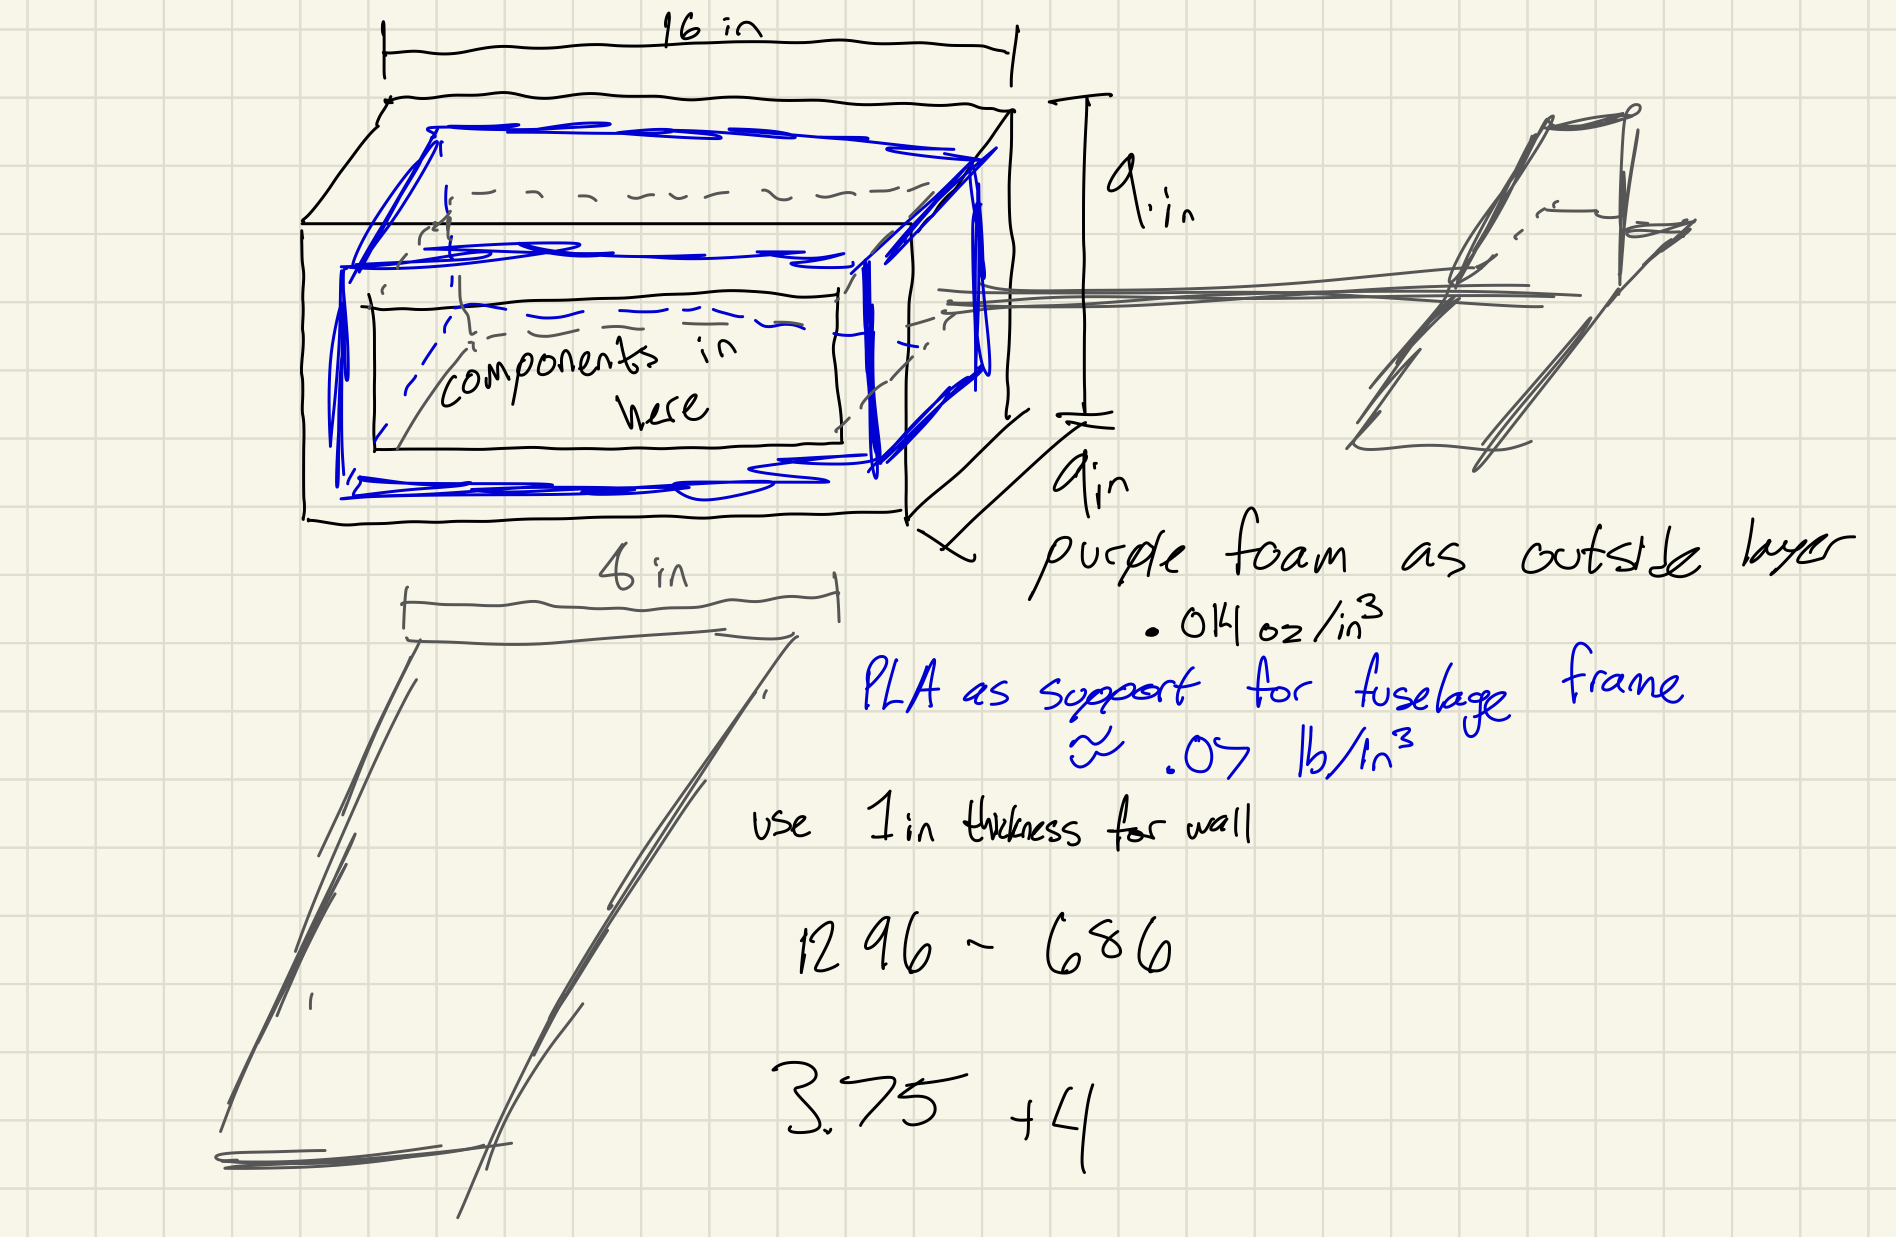
\includegraphics[width=\linewidth]{Figures/fuselage_sketch.png}
    \caption[Fuselage sketch]{A sketch of the fuselage frame and dimensions.}
    \label{fig:fuselage_sketch}
\end{figure}
